Para que pudéssemos aplicar corretamente o filtro, foi necessário o cálculo da ordem do mesmo, bem como a atenuação da banda passante ($\epsilon$).

Foram definidos os seguintes parâmetros para o filtro \textit{Elíptico} passa-baixa:

\begin{enumerate}
    \item Banda passante $\omega_p=1000 \, \text{Hz}$
    \item Banda de rejeição $\omega_s = 2000\, \text{Hz}$
    \item Atenuação da banda passante $\alpha_p = 1dB$
    \item Atenuação da banda de rejeição $\alpha_s = 60dB$
\end{enumerate}


\subsubsection*{Executando o cálculo da ordem do filtro}
Incialmente, devemos realizar o cálculo da ordem do filtro, que segue a fórmula:

\begin{align} \
    k = \frac{\omega_p}{\omega_s}                           \\
    u = \frac{1 - \sqrt[4]{1 - k^2}}{2 (1+\sqrt[4]{1-k^2})} \\
    q = u + 2u^5 + 15u^9 + 150u^13                          \\
    D = \frac{10^{\alpha_s/10} - 1}{10^{\alpha_p/10}-1}     \\
    n = \text{ceil} \left( \frac{\log{16D}}{\log{1/q}} \right)
\end{align}

Substituindo e encontrando os valores, temos:

\begin{align*} \
    k = \frac{\omega_p}{\omega_s} \\
    k = \frac{1000}{2000}         \\
    \therefore k = 0.5
\end{align*}

Tendo o valor de $k$, podemos calcular $u$:

\begin{align*} \
    u = \frac{1 - \sqrt[4]{1 - k^2}}{2 (1 + \sqrt[4]{1 - k^2})}     \\
    u = \frac{1 - \sqrt[4]{1 - 0.5^2}}{2 (1 + \sqrt[4]{1 - 0.5^2})} \\
    \\
    u = \frac{1 - 0.9306}{2 (1 + 0.9306)}                           \\
    u = \frac{0.0694}{3.8612}                                       \\
    u =\approx 0.01797
\end{align*}

Com o valor de $u$, calcula-se $q$:

\begin{align*}
    q = u + 2u^5 + 15u^9 + 150u^{13}                                                     \\
    q = 0.01797 + 2(0.01797)^5                                                           \\
    \quad + 15(0.01797)^9 + 150(0.01797)^{13}                                            \\
    \\
    q = 0.01797 + 2 \cdot (1.8790937 \times 10^{-9})                                     \\
    \quad + 15 \cdot (1.9638449 \times 10^{-16}) + 150 \cdot (2.0524186 \times 10^{-23}) \\
    \\
    q = 0.01797 + 3.7581874 \times 10^{-9}                                               \\
    \quad + 2.9457674 \times 10^{-15} + 3.0786279 \times 10^{-21}                        \\
    \\
    q \approx 0.017970003758190345
\end{align*}


Como os termos menores são extremamente pequenos, podemos considerar $q=u$ no cálculo final de $n$.
Porém antes de calcular $n$, devemos encontrar $D$:

\begin{align*} \
    D = \frac{10^{\alpha_s / 10} - 1}{10^{\alpha_p / 10} - 1} \\
    D = \frac{10^{60 / 10} - 1}{10^{1 / 10} - 1}              \\
    D = \frac{10^{6} - 1}{1.25892541179 - 1}                  \\
    D = \frac{999999}{0.25892541179}                          \\
    D \approx 3862112.23
\end{align*}

Por fim, temos que:

\begin{align*} \
    n = \text{ceil} \left( \frac{\log{16D}}{\log{1/q}} \right)                                    \\
    n = \text{ceil} \left( \frac{\log{16 \cdot 3862112.23}}{\log{1/0.017970003758190345}} \right) \\
    n = \text{ceil} \left( \frac{7.79094487255}{1.74545183206} \right)                            \\
    n = \text{ceil} \left( \frac{7.79094487255}{1.74545183206} \right)                            \\
    n = \text{ceil} (4.4635691054)                                                                \\
    \therefore n = 5
\end{align*}

Portanto, é possível definir que o filtro elíptico aplicado terá \textbf{ordem 5}.


\subsubsection*{Cálculo da função de transferência}

Agora que temos a ordem $n = 5$, podemos expressar a função de transferência $H(s)$ para o filtro elíptico passa-baixa.

A forma geral da função de transferência para um filtro elíptico passa-baixa é:

$$
    H(s) = \frac{\prod_{k=1}^{N} (s - z_k)}{\prod_{k=1}^{M} (s - p_k)} \cdot \text{Ganho}
$$

onde:
\begin{enumerate}
    \item $N$ é o número de zeros,
    \item $M$ é o número de polos (5 neste caso),
    \item $z_k$ são os zeros da função de transferência,
    \item $p_k$ são os polos da função de transferência.
\end{enumerate}

\begin{lstlisting}[language=Octave]
% n = ordem, Rp = ripple na banda passante (em dB)
% Rs = atenuacao na banda de parada (em dB)
% Wp = frequencia de corte normalizada
% 'low' indica filtro passa-baixa
[b, a] = ellip(n, Rp, Rs, Wp, 'low');

% (z) zeros, (p) polos e (k) ganho
[z, p, k] = tf2zp(b, a);
figure;
zplane(z, p);  % Plot
title('Polos e Zeros do Filtro Eliptico');
\end{lstlisting}

A execução do código apresentado permitiu a obtenção dos zeros, polos e do ganho do filtro elíptico, que são elementos fundamentais para a análise e caracterização da sua função de transferência. A Figura \ref{fig:elliptic_zeros_and_poles} apresenta a distribuição dos zeros e polos no plano complexo, destacando a sua relação com as propriedades do filtro.

\begin{figure}[H]
    \centering
    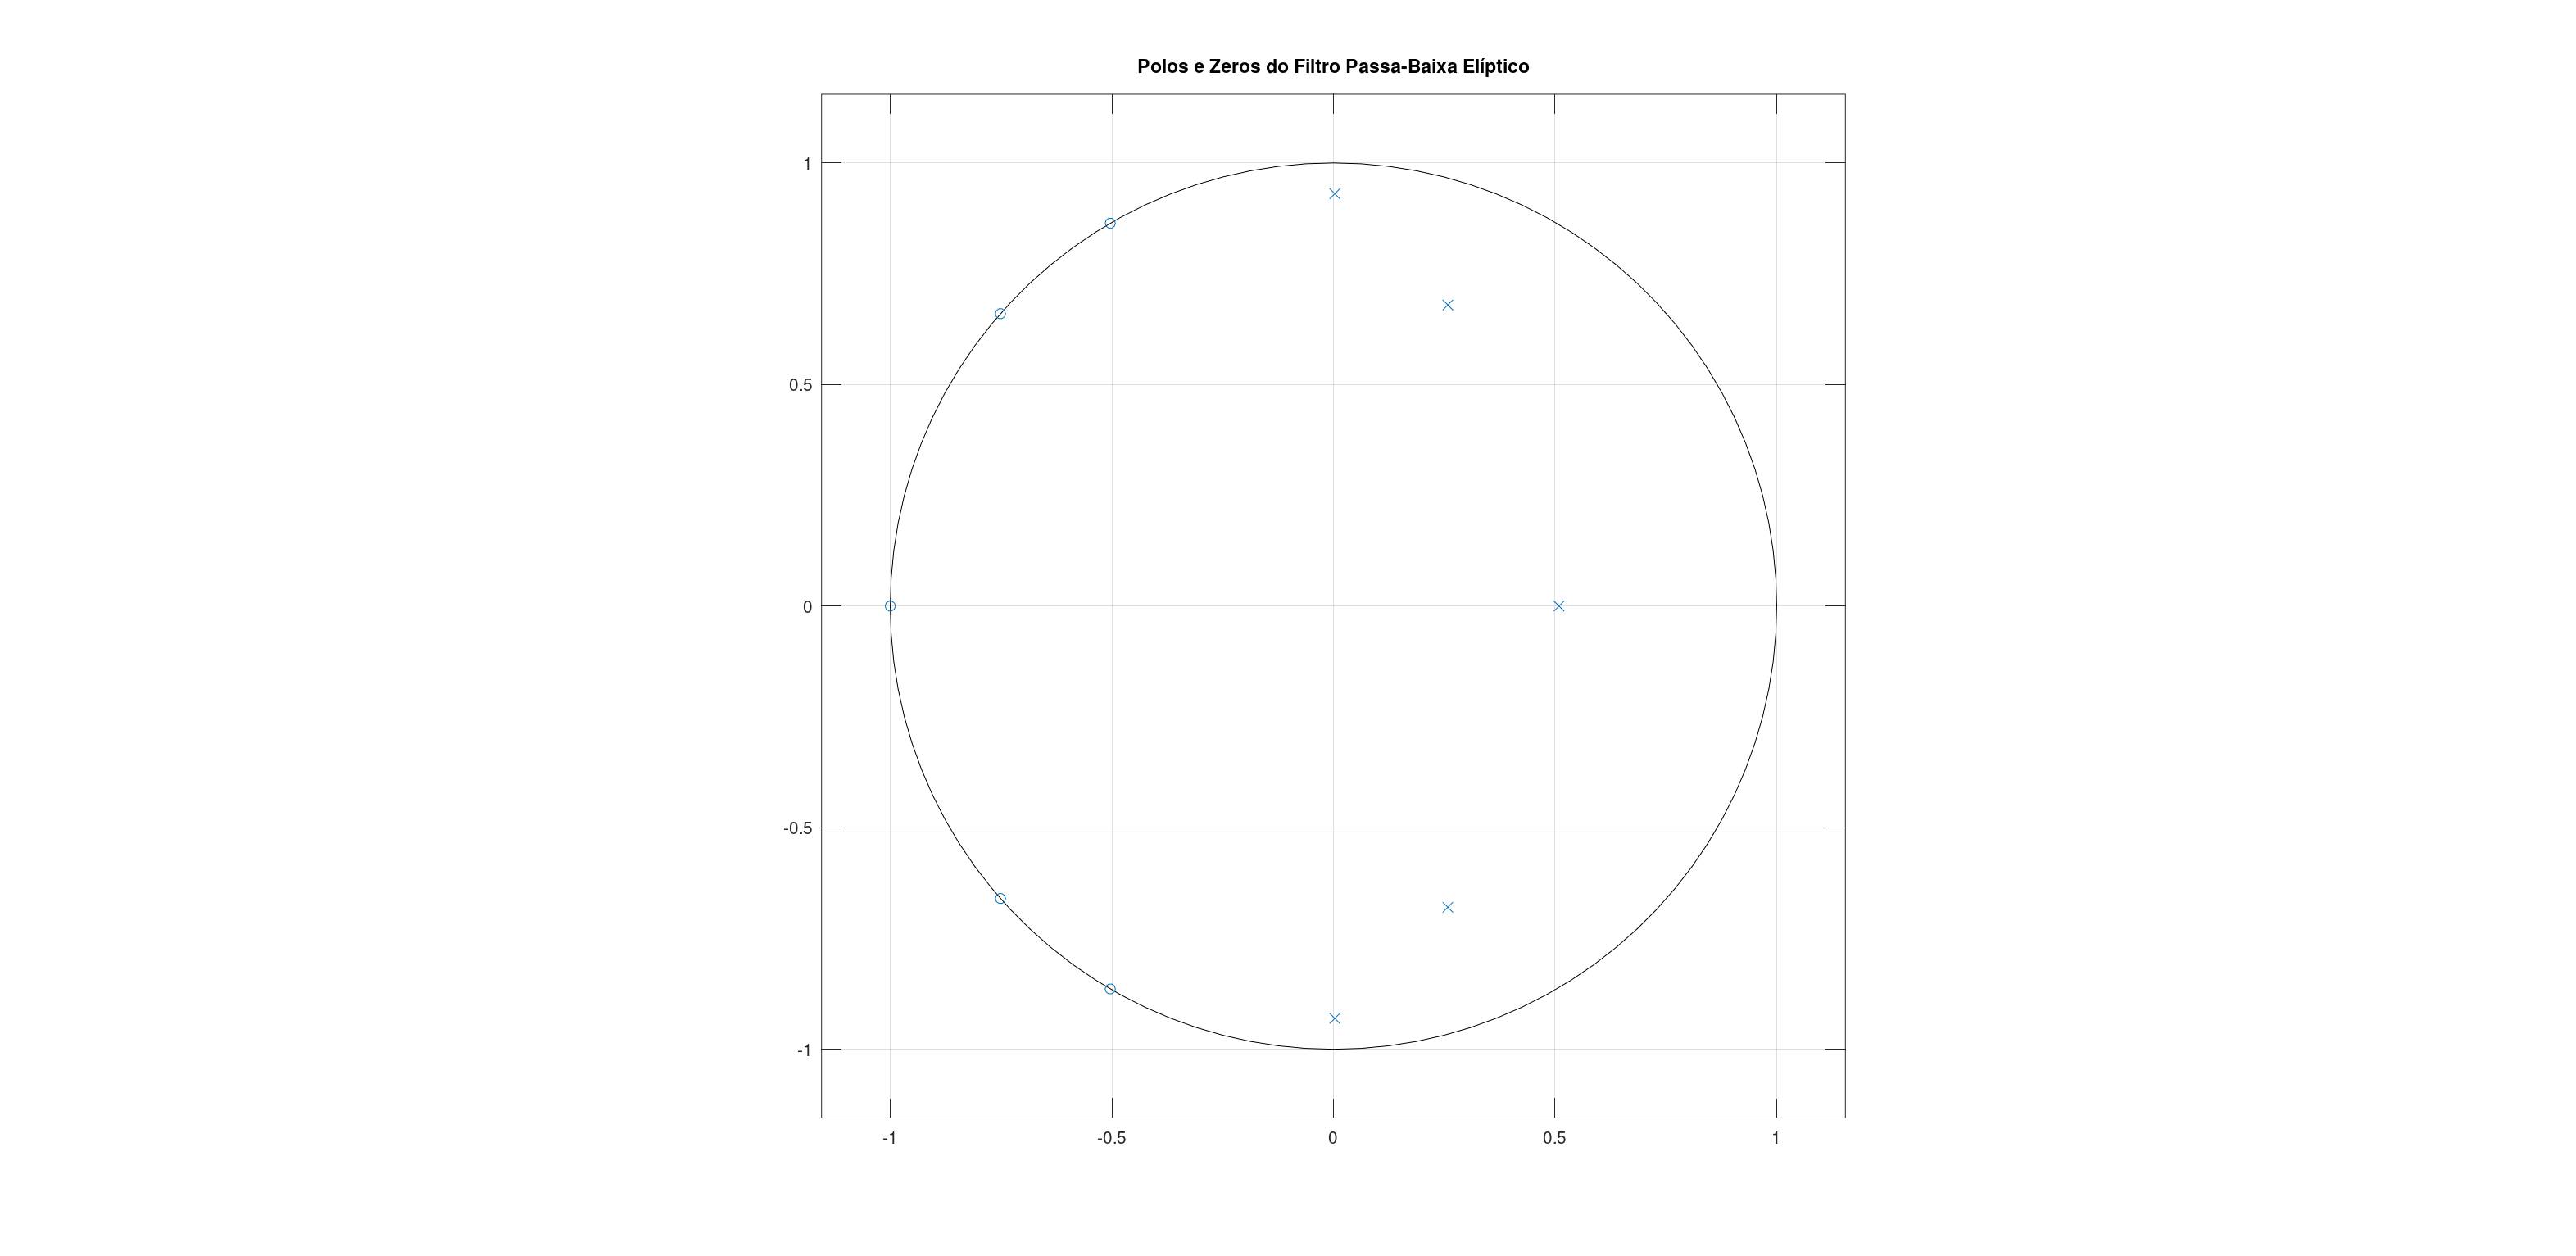
\includegraphics[width=1\linewidth]{02_analytic_development/assets/elliptic_zeroes_and_poles.png}
    \caption{Zeros, polos e ganho obtidos a partir da execução do código do filtro elíptico.}
    \label{fig:elliptic_zeros_and_poles}
\end{figure}

Portanto a função de transferência final do filtro é:
\begin{align*}
    H(s) = \frac{(s + 1)(s + 0.5037 - 0.8639i)}{(s - 0.0030 - 0.9304i)(s - 0.0030 + 0.9304i)}                     \\
    \quad \cdot \frac{(s + 0.5037 + 0.8639i)(s + 0.7514 - 0.6599i)}{(s - 0.2580 - 0.6795i)(s - 0.2580 + 0.6795i)} \\
    \quad \cdot \frac{(s + 0.7514 + 0.6599i)}{(s - 0.5088)}                                                       \\
    \quad \cdot 0.043890
\end{align*}
